\section{\system{} Protocol}
\label{sec:protocol}
Based on the design decisions discussed in the previous section, we specify the 
steps taken to publish and retrieve content in \system{}.

\subsection{Publishing Content}
\label{sec:publish_protocol}
In order to publish content such that the CDN never sees the content, the publisher 
must first obfuscate her content, as described in Section \ref{sec:obfuscate_content}. 
Figure \ref{fig:publishing} shows the steps taken when publishing content.

\begin{figure*}[t]
    \centering
    \begin{subfigure}[h]{0.5\textwidth}
        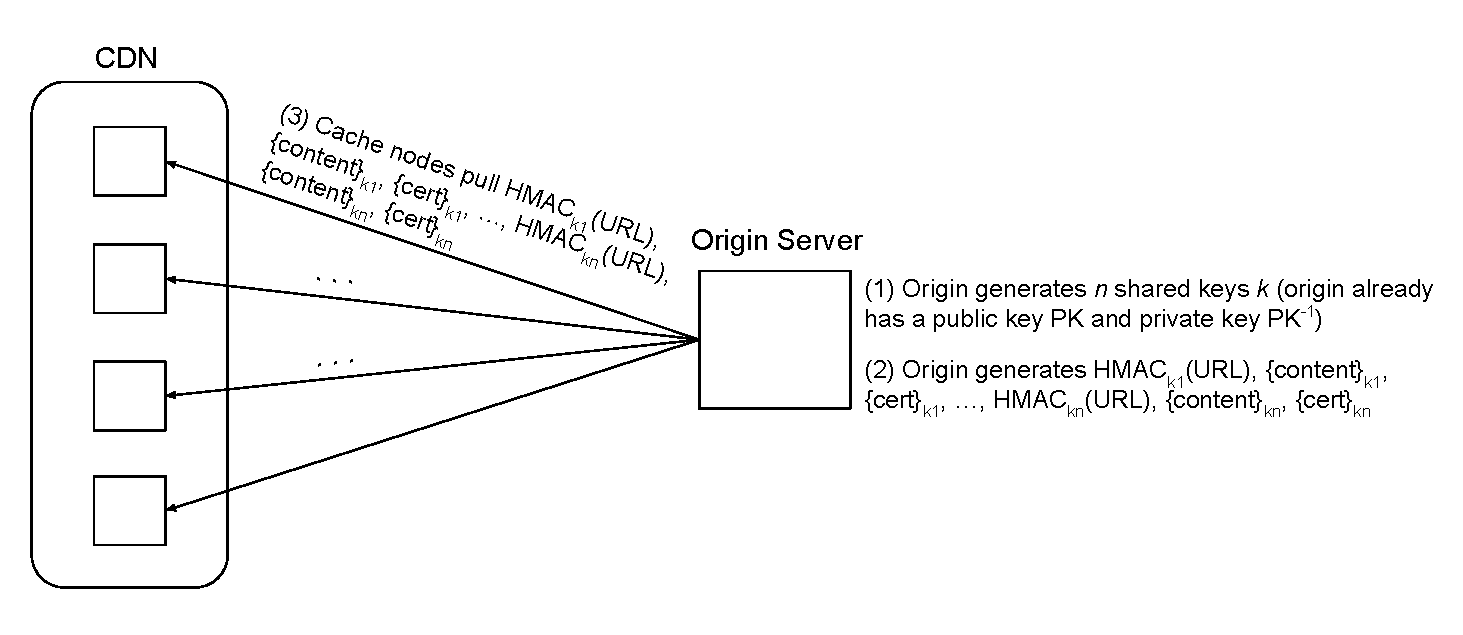
\includegraphics[width=\textwidth]{publishing_content}
    \end{subfigure}%
    \begin{subfigure}[h]{0.5\textwidth}
        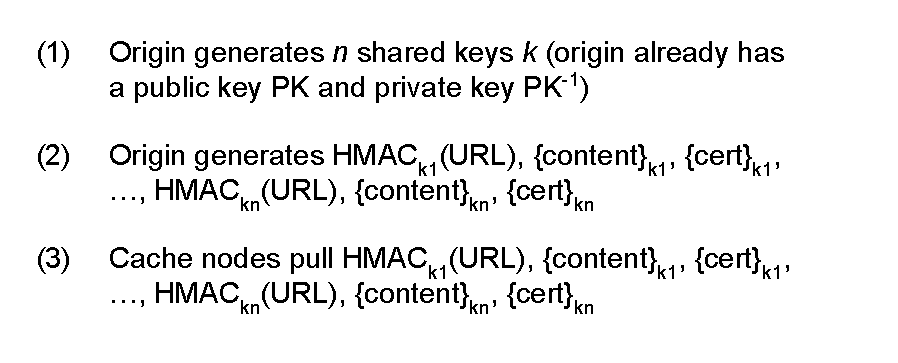
\includegraphics[width=\textwidth]{Publishing_steps}
    \end{subfigure}
    \caption{Step-by-step instructions on how content is published in \system{}.}
    \label{fig:publishing}
\end{figure*}

The most important step in content publishing is obfuscating the data.  We assume that the origin 
server already has a public and private key pair, as well as a certificate.  To obfuscate the data 
the origin server will need to generate $n$ shared keys, where $n$ should be between 1 and the number of 
proxies.  We evaluate the performance tradeoffs of different values of $n$ in Section \ref{sec:performance}.  

Once all keys are established, the publisher must first pad the content to the same size for some 
range of original content sizes (i.e., if content is between length x and y, then pad it to length 
z).  The range of content sizes should be small, such that this causes negligible padding overhead, but 
reduces the linkability between exact content length and content identification.  This content padding is done to hide the original content's length, as it may be identifiable 
simply by its length.  After content is padded, then the content is divided into fixed size blocks and padded to 
some standard length.  Then for each shared key $k$, each block is encrypted using the shared key, 
such that there are $n$ sets of encrypted blocks. As long as the CDN does not have access to any 
of the $n$ shared keys, then the CDN cannot see what content it is caching.  

Now that the content is obfuscated, the publisher must also obfuscate the content's identifier.  To do so, 
she computes the HMAC of the URL using the shared key $k$, for each shared key.

Once the identifier and the content replicas are obfuscated $n$ times (with $n$ keys), they can be pushed to the 
CDN.  Recently, services have cropped up to allow and help facilitate the use of multiple CDNs for the same content; a content 
publisher could use multiple CDNs' services.  This mechanism could be used in \system{} to increase reliability, 
performance, and availability; a publisher can use a service, such as Cedexis~\cite{cedexis}, to load balance between 
CDNs.  We discuss the use of multiple CDNs more in Section \ref{sec:partial} on \system{} in 
partial deployment.  Note that each proxy will only be able to fetch a specific replica of the content, that is a 
specific \{content\}$_{kn}$ for the $n^{th}$ shared key that it holds.  We discuss the performance trade offs 
associated with differing numbers of shared keys and proxies in Sections \ref{sec:performance}.

%\begin{enumerate}
%\item Origin generates n shared keys k (origin already has a public key PK and private key PK$^{-1}$)\footnote{$n$ such that $1 < n < |proxies|$} 
%\item Origin generates HMAC$_{k1}$(URL), \{content\}$_{k1}$, , \{cert\}$_{k1}$, ..., HMAC$_{kn}$(URL), \{content\}$_{kn}$, \{cert\}$_{kn}$
%\item Cache node pulls HMAC$_{k1}$(URL), \{content\}$_{k1}$, , \{cert\}$_{k1}$, ..., HMAC$_{kn}$(URL), \{content\}$_{kn}$, \{cert\}$_{kn}$\footnote{For more security and reliability, cache nodes from different CDNs can pull this data.  Additionally, an origin server can use something like Cedexis to load balance between CDNs.}
%\end{enumerate}

{\bf Updating Content}
For a content publisher to update content, she must follow similar steps as described in publishing content.  
Once she has updated the content on her origin server, she must obfuscate it using the same steps: 1) padding the 
original content length, 2) divide the content into fixed size blocks, and 3) encrypt $n$ copies of the content blocks 
with each of the shared keys.  Because she is updating the content (as opposed to creating new content), the 
obfuscated identifier will remain the same.  She must 
retain a copy of the obfuscated old content until after the new content has been updated on the CDN; this is to prove 
that the old content owner is the same as the new content owner.  The CDN cannot simply authenticate the content publisher, as this 
typically requires some type of identification for the content publisher; the CDN does not need to know --- and should not know --- 
the identity of the publisher, just that the organization that originally published the content is the same as the one that is 
updating the content.  Only the origin and the proxy, both of which are 
outside the CDN, know the old obfuscated content, so an attacker cannot update the content that belongs to 
a legitimate publisher.  The publisher must present the old obfuscated content to the CDN in order to also push 
her new obfuscated content to the CDN. 

\subsection{Retrieving Content}
The steps taken for an end-user to retrieve a web page that has been cached by \system{} are shown in Figure \ref{fig:retrieving}.  
The end-user must first configure her browser to use an \system{}-designated proxy, meaning a proxy that is a part of the system, but not controlled by the 
CDN provider.  A client is assigned to a 
specific proxy based on her location, and she configures her browser to use the assigned proxy.    Then, once she sends a request for a 
web page, it goes to the proxy via a TLS connection.\footnote{Comment: Add blinding here such that client1's request for foo.com and 
client2's request for foo.com looks different as it goes from the client to the proxy.  So the proxy must be able to un-blind 
the request.}  The proxy then resolves the domain using it's local resolver, which will 
redirect it to the CDN's DNS resolver. 

In order for the proxy to generate the obfuscated identifier to query the edge server for the correct content, 
it must have one of the $n$ shared keys that the origin server generated and obfuscated the content and identifier 
with.  The origin server publishes the shared key encrypted with the proxy's public key\footnote{Additionally, the origin server 
can learn the proxy's public key via DNS as well; for example, the proxy can publish it's public key in the DNS SRV record.} in the DNS SRV record; therefore, 
when the proxy sends a DNS request to the origin server's authoritative DNS server, it will receive the encrypted shared 
key, which it can decrypt with it's private key.  Because the list of \system{} proxies is publicly available, it is simple for a 
content publisher to retrieve the list of proxies and ensure that she encrypts the shared key with each proxy's public key.

Now that the proxy has obtained a shared key from the origin server, it can generate the obfuscated content identifier based 
on the request the client sent.  It computes the HMAC of the URL with the shared key.  The proxy then 
sends the (obfuscated) request to the edge server, where the CDN locates the content associated with the identifier.  The CDN returns 
the associated obfuscated content, which we recall is the fixed size blocks encrypted with the same shared key that the identifier was 
obfuscated with.  The proxy can decrypt the content blocks with the shared key from the origin server, assemble the blocks, and strip any 
added padding, to reconstruct the original content.\footnote{Comment: Proxy can cache content in times of flash crowd to minimize correlation attacks if a provider has encrypted and unencrypted content on the same CDN.  This raises the issue of charges for the origin (the CDN can’t charge as much if edge servers don’t see as many requests for the origin) --- RFC 2227 describes a solution for this~\cite{rfc2227}.}  Finally, the proxy returns the content to the client over TLS.  

%\begin{enumerate}
%\item Send GET foo.com request to proxy using TLS connection\footnote{Include some form of blinding here such that client1 and client2 request the same URL, but the contents of step 1 look different by adding some randomness at the client, and that the proxy can remove \url{https://en.wikipedia.org/wiki/Blinding_(cryptography)} --- this prevents a malicious CDN from running a client and sending requests to learn things about other clients.}
%\item DNS lookup from proxy for foo.com\footnote{This DNS info could be prefetched on the proxy, which would provide some optimization.}
%\item CDN DNS lookup for a19.akamai.net (some Akamai ID that represents foo.com)
%\item Proxy sends DNS request to origin’s authoritative server, and the origin publishes \{k\}$_{PK_{proxy}}$ in the SRV record.  Then the proxy decrypts the shared key with his own private key.\footnote{The origin can learn the proxy’s public key via DNS.}, \footnote{The shared keys are updated every X amount of time, so this fetching of the shared key needs to happen regularly.}
%\item Proxy generates GET HMAC$_k$(URL) request
%\item Proxy sends request to cache node
%\item Cache node returns \{content\}$_k$, \{cert\}$_k$ to proxy.  Proxy decrypts and validates the cert.  Once the cert is validated, proxy decrypts the content with origin server’s shared key.\footnote{Proxy can cache content in times of flash crowd to minimize correlation attacks if a provider has encrypted and unencrypted content on the same CDN. This raises the issue of charges for the origin (the CDN can’t charge as much if edge servers don’t see as many requests for the origin) --- RFC 2227 describes a solution for this: Simple Hit-Metering and Usage-Limiting for HTTP.}
%\item Proxy returns decrypted content to client (using TLS)
%\end{enumerate}

\begin{figure*}[t]
    \centering
    \begin{subfigure}[h]{0.5\textwidth}
        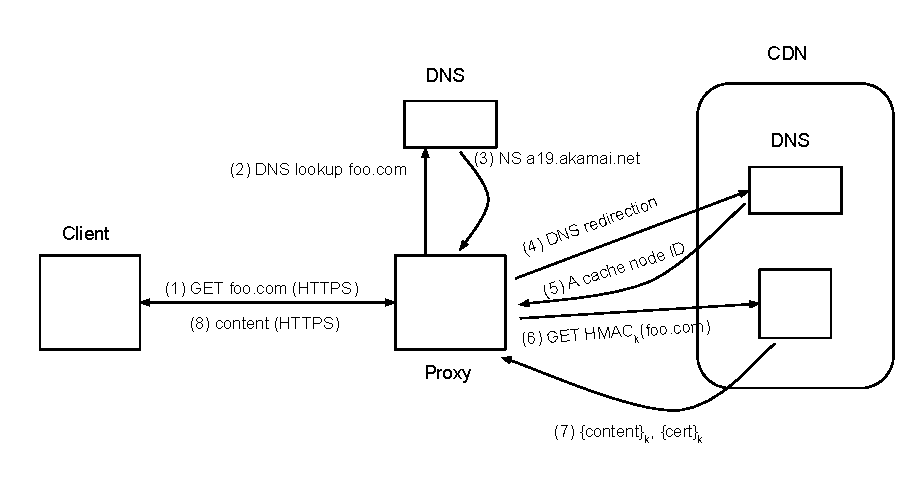
\includegraphics[width=\textwidth]{retrieving_content}
    \end{subfigure}%
    \begin{subfigure}[h]{0.5\textwidth}
        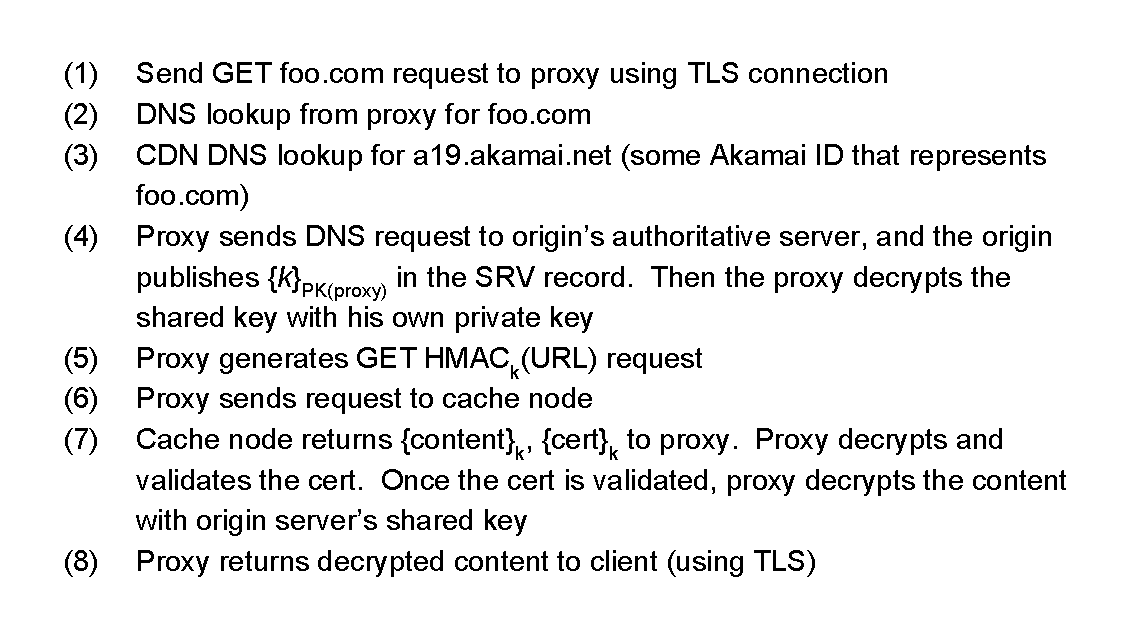
\includegraphics[width=\textwidth]{Retrieving_steps}
    \end{subfigure}
    \caption{Step-by-step instructions on how content is retrieved in \system{}.}
    \label{fig:retrieving}
\end{figure*}

\subsection{Partial Deployment}
\label{sec:partial}
\system{} should be partially deployable in the sense that if only some of the content publishers participate or only some of the CDNs participate, then 
the system should still provide protections.  We have two different partial deployment plans, and both provide protections for those 
publishers, CDNs, and clients that use \system{}. 

\paragraph{Deployment Option 1.}
One option for deploying \system{} is to ensure there is some set $S$ of content publishers the participate fully in the 
system.  These publishers obfuscate their content, identifiers, and certificates, and most importantly, only have 
obfuscated data stored on the CDNs cache nodes.  Recall that there are $n$ shared keys, resulting in $n$ replicas of the 
content that {\it appear} to the CDN as different content (because each replica is encrypted with a different key).  This 
allows the minimum set of publishers $S$ to be relatively small; $S$ must be greater than one, otherwise the CDN can infer 
that a client accessing this obfuscated content is actually accessing content that can be identified.  This partial deployment plan 
partially protects the privacy of the clients accessing the content created by the set of publishers $S$.  It does not 
protect the clients' privacy as completely as full participation of all publishers in \system{} because the CDN can 
still view cross site browsing patterns among the publishers that are not participating. It is important to note though, that 
because the clients are behind proxies, the CDN cannot individually identify users.  The CDN can attribute requests to proxies, but 
not to clients.  

\paragraph{Deployment Option 2.} 
It is reasonable to believe that some content publishers are skeptical of \system{} and prioritize performance 
and availability.  Therefore, they should have the option to gradually move towards full participation by pushing 
both encrypted and plaintext content to the CDN.  In this partial deployment plan, we see some set of publishers 
fully participating with only encrypted content, some other set of publishers partially participating with both 
encrypted and plaintext content, and some last set of publishers that are not participating.  Unfortunately, if 
a publisher has both encrypted and plaintext content at a cache node, and some event causes a flashcrowd --- 
the CDN sees a significantly larger spike in accesses to certain content --- then the CDN can correlate the access 
spike on encrypted and plaintext content for the same publisher.  In order to prevent this deanonymization of the 
content publisher, we can utilize multiple CDNs.  The publisher can spread replicas over different CDNs such that 
the encrypted replicas are on one CDN and the plaintext replicas are on a different CDN.  In this case the publisher 
is not susceptible to flashcrowds correlations and can still join the system.

\subsection{Optimizations}
\label{sec:optimizations}
While there are some optimizations that CDNs typically perform today that would not be possible with \system{}, the architecture 
of \system{} allows for new optimizations that are not possible in existing CDNs.  Here we describe how \system{} limits 
current traditional CDN's optimizations, and then we outline some ways in which \system{} 
can be optimized in terms of performance.

CDNs become slightly limited in terms of the possible performance optimizations when following \system{}'s design.  For example, 
many CDNs perform HTTPS re-writes on content that they cache, but this can only be done if the CDN has access to the 
decrypted content.  Similarly, the CDN needs the decrypted content to perform minimizations on HTML, CSS, and Javascript 
files.  While this likely increases performance in traditional CDNs, it does not provide the greatest increase in performance; 
content caching around the world is the greatest benefit to performance, which \system{} preserves.

\paragraph{Pre-Fetch DNS Responses.} One way to increase the performance of \system{} is to pre-fetch DNS responses at 
the proxies.  This would allow the proxy to serve each client request faster because it would not have to send 
as many DNS requests.  Pre-fetching DNS responses would not take up a large amount of space, but it also 
would not be a complete set of all DNS responses.  Additionally, if the content is moved between cache nodes 
at the CDN, then DNS response must also change; therefore, the pre-fetched DNS responses should have a 
lifetime that is shorter than the lifetime of the content on a cache node.

\paragraph{Load Balance Proxy Selection.} As the proxy performs a number of operations on the client's behalf, it 
runs into the possibility of being overloaded.  With \system{}, a client can be redirected to different 
proxies based on load; this can be implemented with a PAC file, which allows 
a client to access different proxies for different domains.  In addition to being a performance benefit, 
this could also prevent a country from blocking the set of proxies that all of the country's citizens use; if 
this occurs, then the citizens can be redirected to a different proxy.   
